\documentclass[oneside]{VUMIFPSkursinis}
\usepackage{algorithmicx}
\usepackage{algorithm}
\usepackage{algpseudocode}
\usepackage{amsfonts}
\usepackage{float}
\usepackage{amsmath}
\usepackage{bm}
\usepackage{caption}
\usepackage{color}
\usepackage{float}
\usepackage{graphicx}
\usepackage{listings}
\usepackage{subfig}
\usepackage{ltablex}
\usepackage{longtable}
\usepackage{wrapfig}
\usepackage{subfig}
\usepackage{pbox}
\renewcommand{\labelenumii}{\theenumii}
\renewcommand{\theenumii}{\theenumi.\arabic{enumii}.}
\renewcommand{\labelenumiii}{\theenumiii}
\renewcommand{\theenumiii}{\theenumii\arabic{enumiii}.}
\newcolumntype{P}[1]{>{\centering\arraybackslash}p{#1}}
\usepackage[%  
    colorlinks=true,
    linkcolor=black
]{hyperref}
\university{Vilniaus universitetas}
\faculty{Matematikos ir informatikos fakultetas}
\department{Programų sistemų katedra}
\papertype{Programų sistemų inžinerija II laboratorinis darbas II}
\title{Reikalavimų analizė ir techninė architektūra}
\titleineng{Requirements Analysis and Technical Architecture}
\status{2 kurso 3 grupės studentai}



\supervisor{Audronė Lupeikienė, M. Darbuot., Dr.}
\date{Vilnius – \the\year}

\bibliography{bibliografija}

\begin{document}
\maketitle
\tableofcontents

\section{Anotacija}
\begin{itemize}
	\item{Matas Savickis}
	\item{Justas Tvarijonas}
	\item{Rytautas Kvasinskas}
	\item{Greta Pyrantaitė}
	\item{Tomas Kiziela}
\end{itemize}

\section{Sistemos detalus projektas}
	\subsection{Sistemos užduotys}
		\subsubsection{Užduočių diagramos}


			\begin{figure}[h]
    				\centering
    				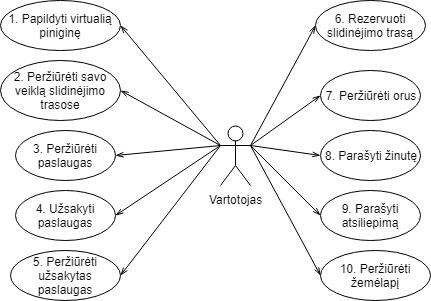
\includegraphics[width=0.75\textwidth]{useCaseVartotojas.png}
    				\caption{Vartotojo užduočių diagrama}
    				\label{fig:VartotojoUseCasel}
			\end{figure}

			\begin{figure}[h]
    				\centering
    				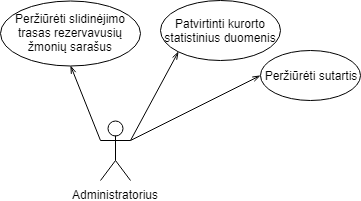
\includegraphics[width=0.75\textwidth]{useCaseAdministratorius.png}
    				\caption{Vartotojo užduočių diagrama}
    				\label{fig:VartotojoUseCasel}
			\end{figure}
\pagebreak

	\subsubsection{Robastiškumo diagramos}

			\begin{figure}[h]
    				\centering
    				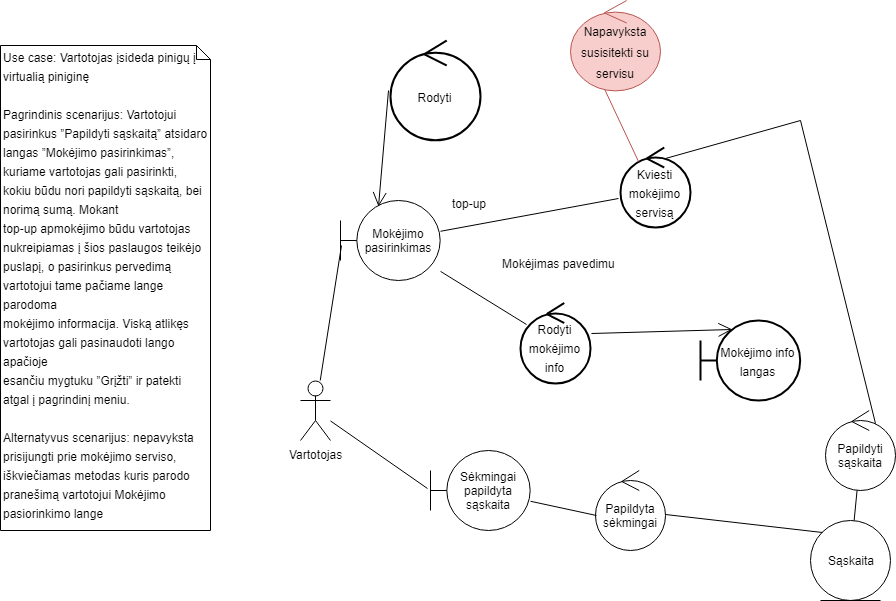
\includegraphics[width=0.75\textwidth]{rob1.png}
    				\caption{Vartotojas įsideda pinigų į virtualią piniginę}
    				\label{fig:Vartotojas įsideda pinigų į virtualią piniginę}
			\end{figure}

			\begin{figure}[h]
    				\centering
    				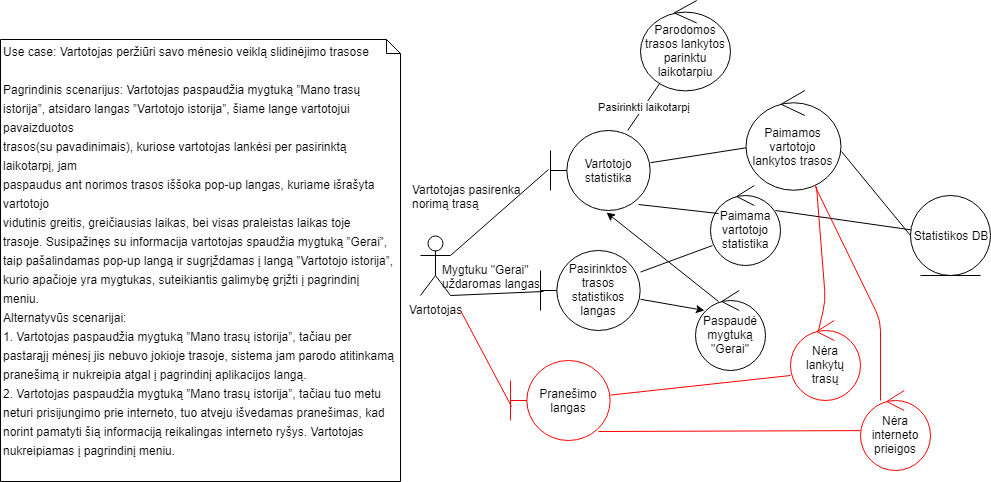
\includegraphics[width=0.75\textwidth]{rob2.png}
    				\caption{Vartotojas peržiūri savo veiklą trasose}
    				\label{fig:Vartotojas peržiūri savo veiklą trasose}
			\end{figure}

			\begin{figure}[h]
    				\centering
    				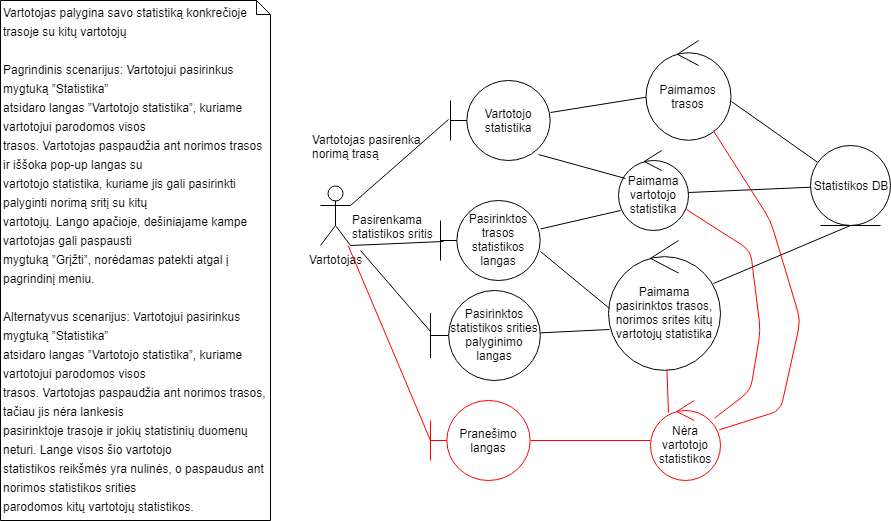
\includegraphics[width=0.75\textwidth]{rob3.png}
    				\caption{Vartotojas palygina savo statistiką trasoje}
    				\label{fig:Vartotojas palygina savo statistiką trasoje}
			\end{figure}

			\begin{figure}[h]
    				\centering
    				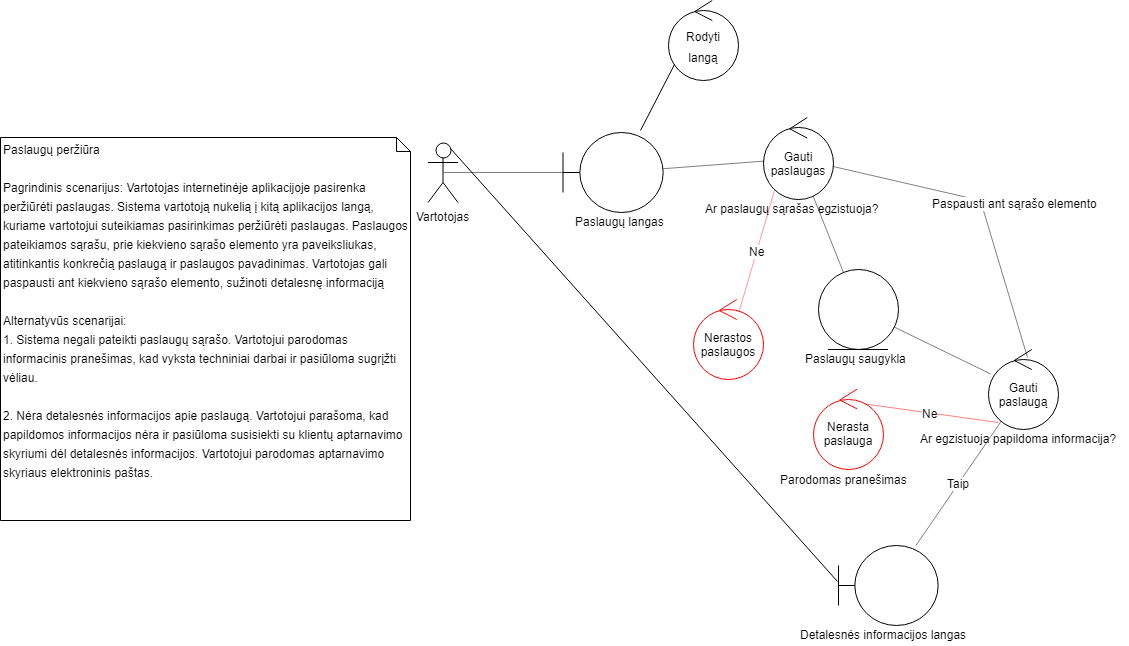
\includegraphics[width=0.75\textwidth]{rob4.png}
    				\caption{Paslaugų peržiūra}
    				\label{fig:Paslaugų peržiūra}
			\end{figure}

			\begin{figure}[h]
    				\centering
    				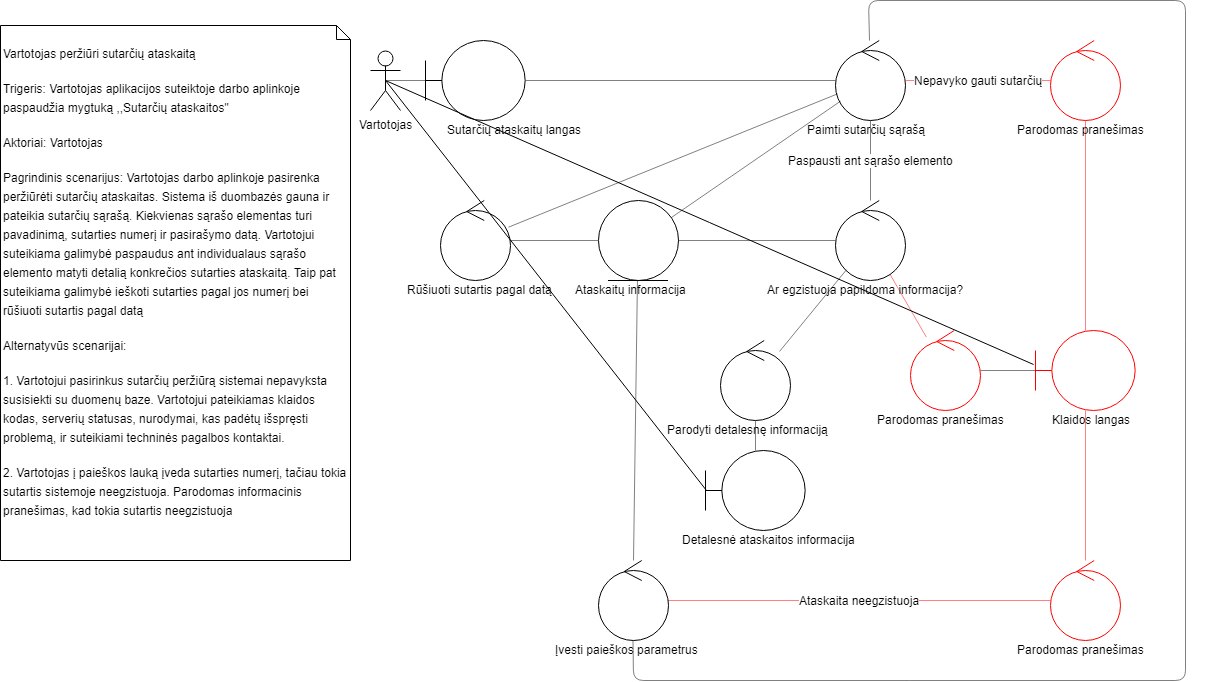
\includegraphics[width=0.75\textwidth]{rob5.png}
    				\caption{Vartotojas peržiūri sutarčių ataskaita}
    				\label{fig:Vartotojas peržiūri sutarčių ataskaita}
			\end{figure}

			\begin{figure}[h]
    				\centering
    				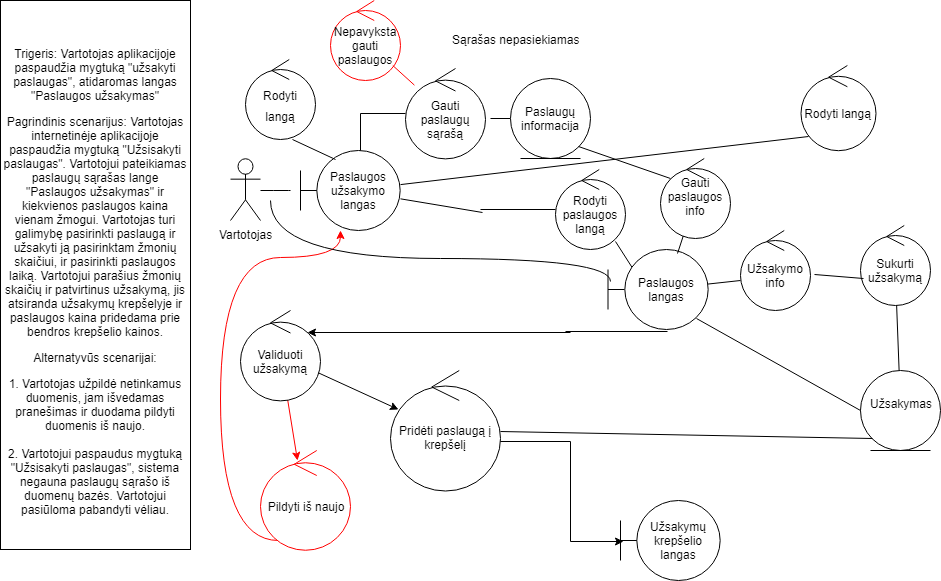
\includegraphics[width=0.75\textwidth]{rob6.png}
    				\caption{Vartotojas užsisako paslaugas}
    				\label{fig:Vartotojas užsisako paslaugas}
			\end{figure}

			\begin{figure}[h]
    				\centering
    				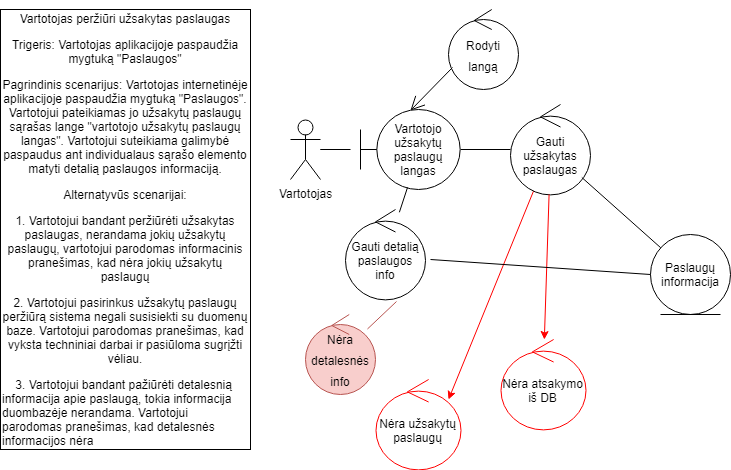
\includegraphics[width=0.75\textwidth]{rob7.png}
    				\caption{Vartotojas peržiūri užsakytas paslaugas}
    				\label{fig:Vartotojas peržiūri užsakytas paslaugas}
			\end{figure}

			\begin{figure}[h]
    				\centering
    				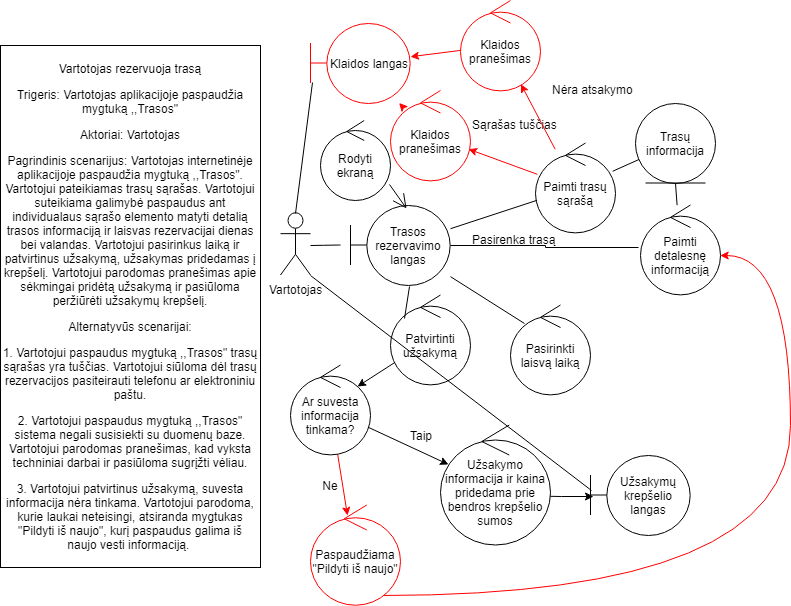
\includegraphics[width=0.75\textwidth]{rob8.png}
    				\caption{Vartotojas rezervuoja trasą}
    				\label{fig:VartotojoUseCasel}
			\end{figure}

			\begin{figure}[h]
    				\centering
    				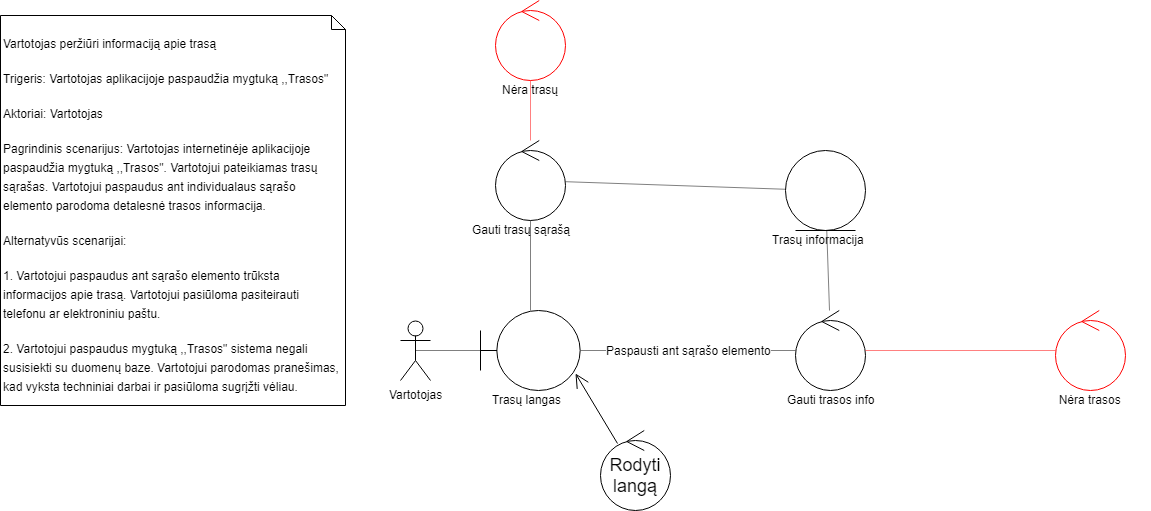
\includegraphics[width=0.75\textwidth]{rob9.png}
    				\caption{Vartotojas peržiūri trasos informacijos}
    				\label{fig:Vartotojas peržiūri trasos informacijos}
			\end{figure}

			\begin{figure}[h]
    				\centering
    				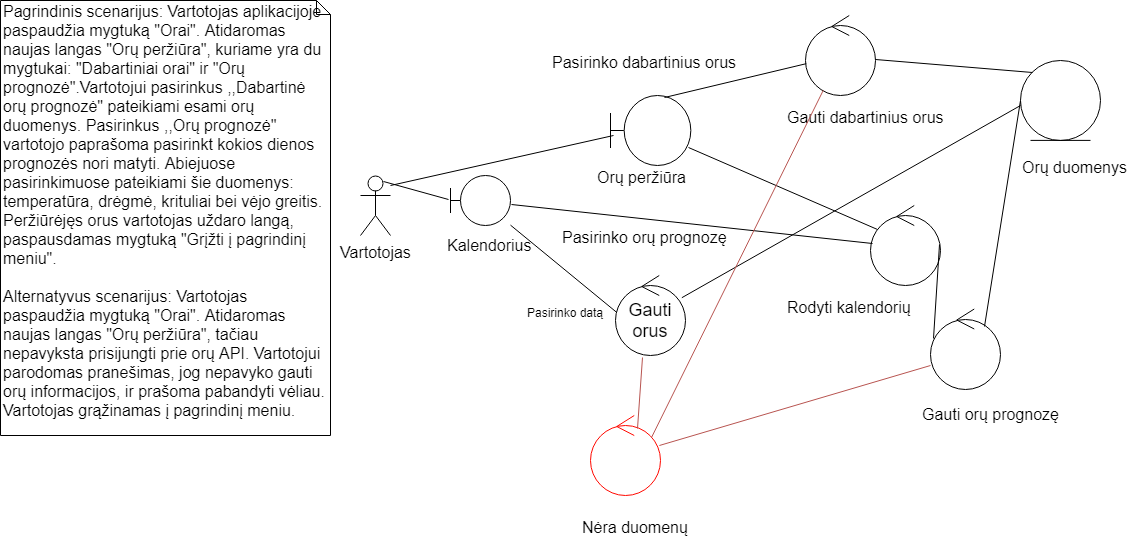
\includegraphics[width=0.75\textwidth]{rob10.png}
    				\caption{Vartotojas peržiūri orų prognozę}
    				\label{fig:Vartotojas peržiūri orų prognozę}
			\end{figure}

			\begin{figure}[h]
    				\centering
    				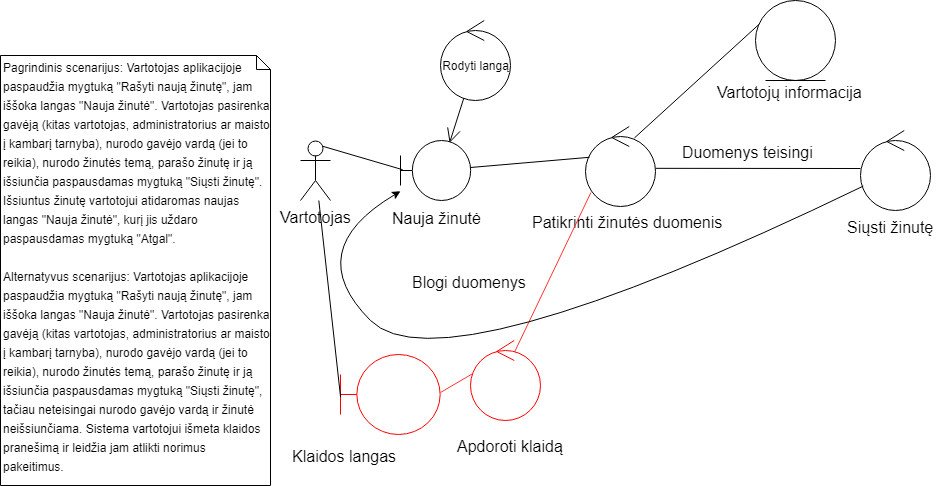
\includegraphics[width=0.75\textwidth]{rob11.png}
    				\caption{Vartotojas rašo žinutę}
    				\label{fig:Vartotojas rašo žinutę}
			\end{figure}

			\begin{figure}[h]
    				\centering
    				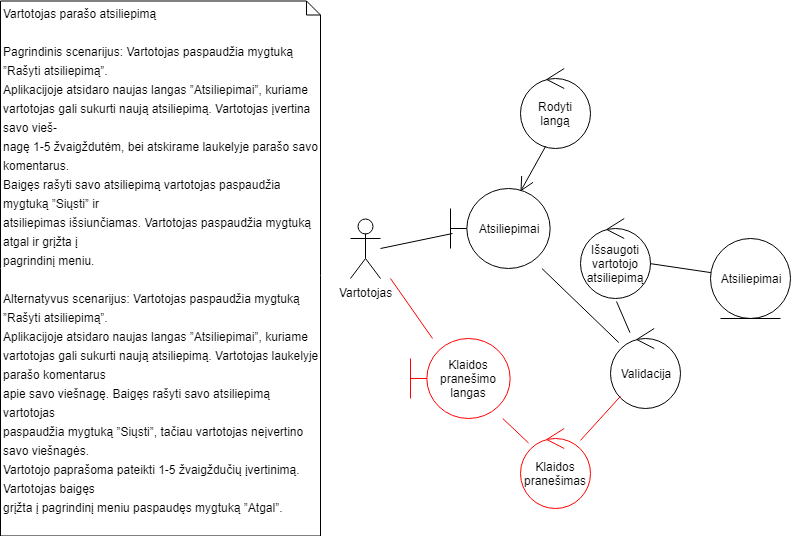
\includegraphics[width=0.75\textwidth]{rob12.png}
    				\caption{Vartotojas rašo atsiliepimą}
    				\label{fig:Vartotojas rašo atsiliepimą}
			\end{figure}

			\begin{figure}[h]
    				\centering
    				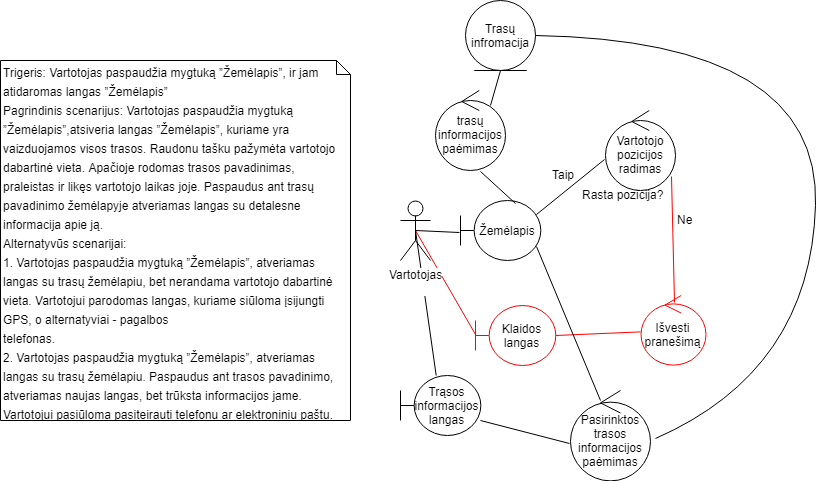
\includegraphics[width=0.75\textwidth]{rob13.png}
    				\caption{Vartotojas peržiūri žemėlapį}
    				\label{fig:Vartotojas peržiūri žemėlapį}
			\end{figure}

			\begin{figure}[h]
    				\centering
    				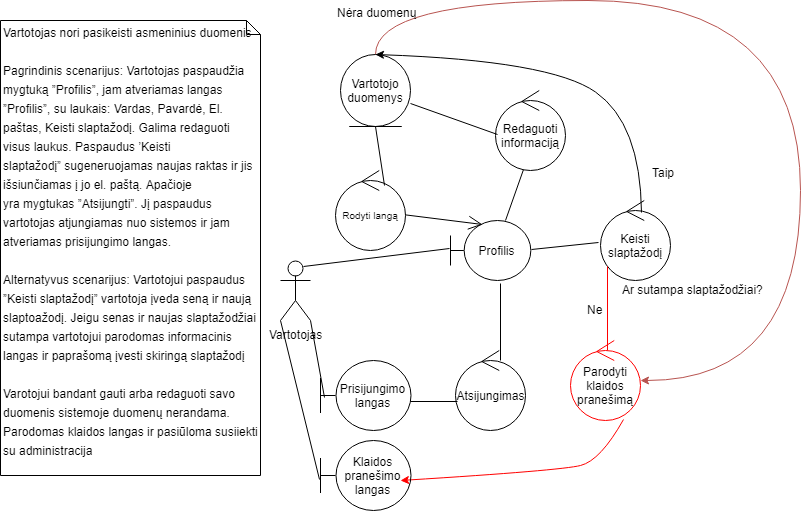
\includegraphics[width=0.75\textwidth]{rob14.png}
    				\caption{Vartotojas keičia asmeninius duomenis}
    				\label{fig:Vartotojas keičia asmeninius duomenis}
			\end{figure}

\section{Sekų diagramos}
			\begin{figure}[h]
    				\centering
    				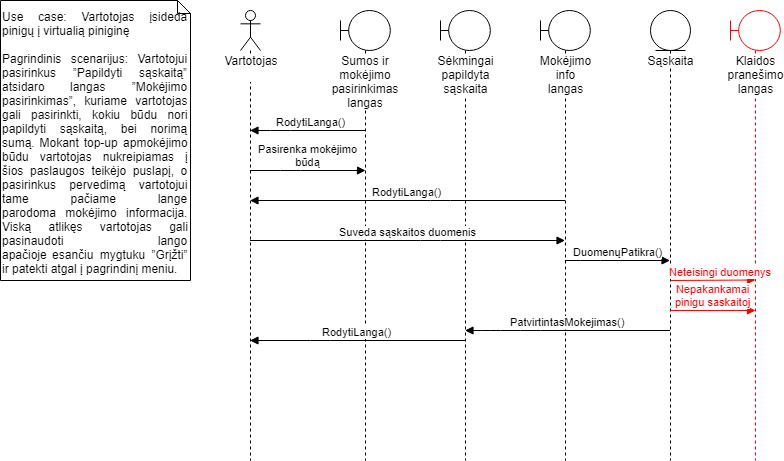
\includegraphics[width=0.75\textwidth]{seq1.png}
    				\caption{Vartotojas įsideda pinigų į virtualią piniginę}
    				\label{fig:Vartotojas įsideda pinigų į virtualią piniginę}
			\end{figure}

			\begin{figure}[h]
    				\centering
    				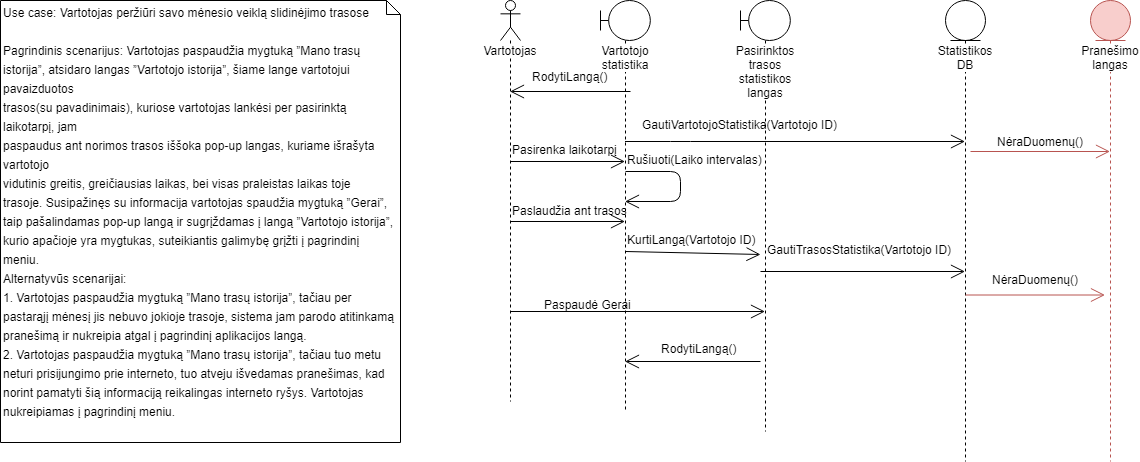
\includegraphics[width=0.75\textwidth]{seq2.png}
    				\caption{Vartotojas peržiūri savo veiklą trasose}
    				\label{fig:Vartotojas peržiūri savo veiklą trasose}
			\end{figure}

			\begin{figure}[h]
    				\centering
    				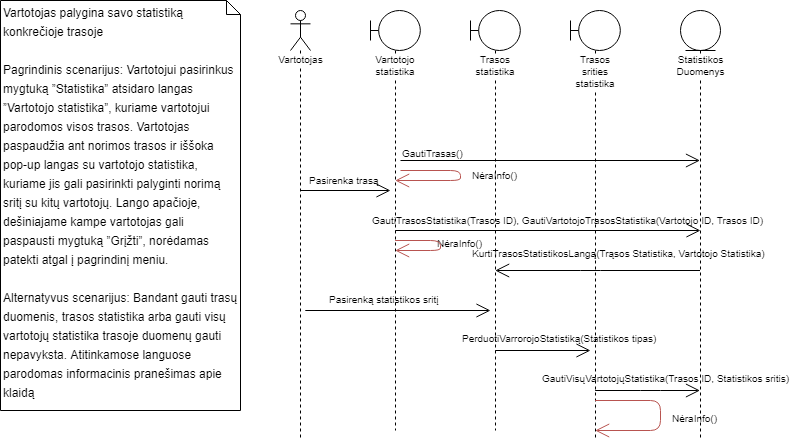
\includegraphics[width=0.75\textwidth]{seq3.png}
    				\caption{Vartotojas palygina savo statistiką trasoje}
    				\label{fig:Vartotojas palygina savo statistiką trasoje}
			\end{figure}

			\begin{figure}[h]
    				\centering
    				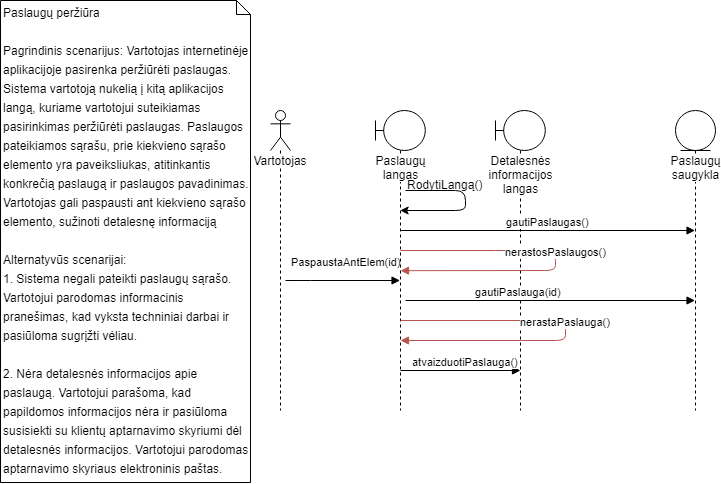
\includegraphics[width=0.75\textwidth]{seq4.png}
    				\caption{Paslaugų peržiūra}
    				\label{fig:Paslaugų peržiūra}
			\end{figure}

			\begin{figure}[h]
    				\centering
    				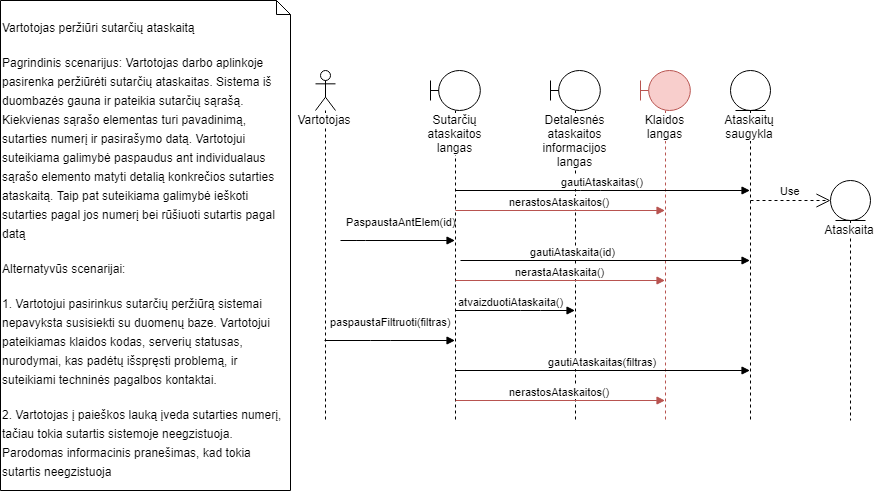
\includegraphics[width=0.75\textwidth]{seq5.png}
    				\caption{Vartotojas peržiūri sutarčių ataskaita}
    				\label{fig:Vartotojas peržiūri sutarčių ataskaita}
			\end{figure}

			\begin{figure}[h]
    				\centering
    				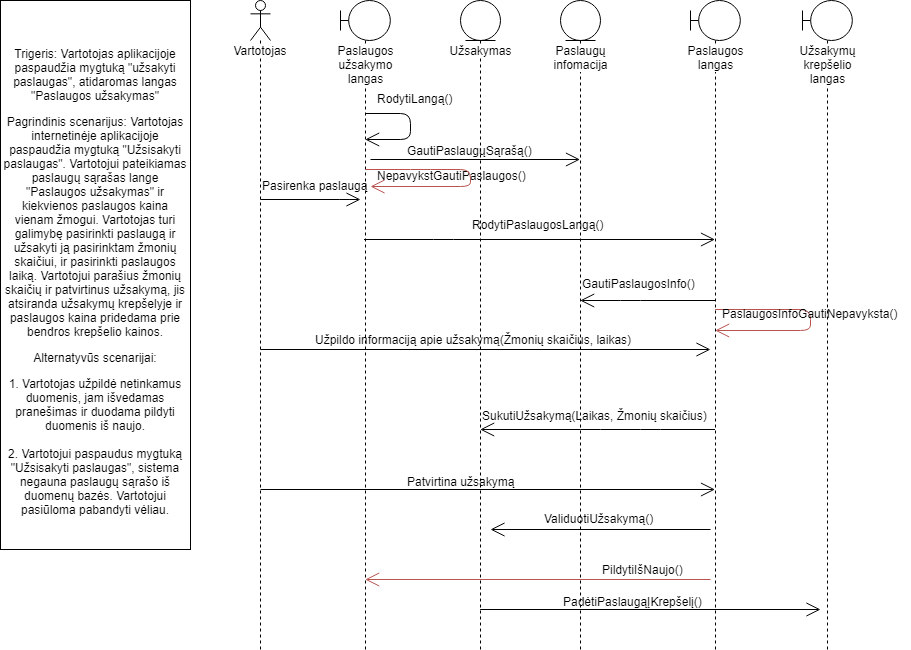
\includegraphics[width=0.75\textwidth]{seq6.png}
    				\caption{Vartotojas užsisako paslaugas}
    				\label{fig:Vartotojas užsisako paslaugas}
			\end{figure}

			\begin{figure}[h]
    				\centering
    				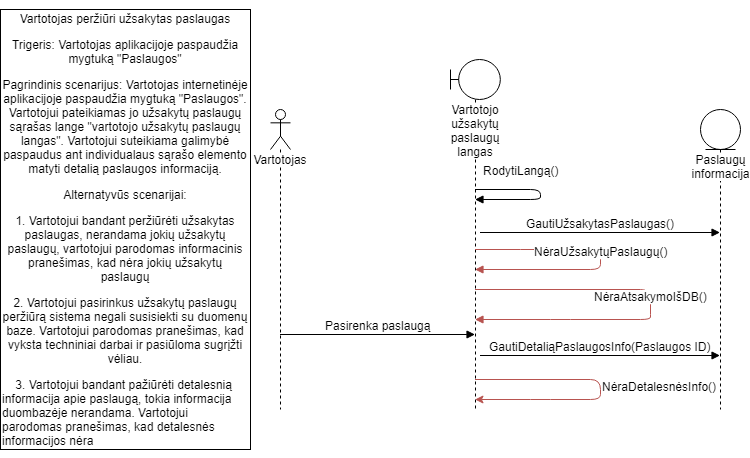
\includegraphics[width=0.75\textwidth]{seq7.png}
    				\caption{Vartotojas peržiūri užsakytas paslaugas}
    				\label{fig:Vartotojas peržiūri užsakytas paslaugas}
			\end{figure}

			\begin{figure}[h]
    				\centering
    				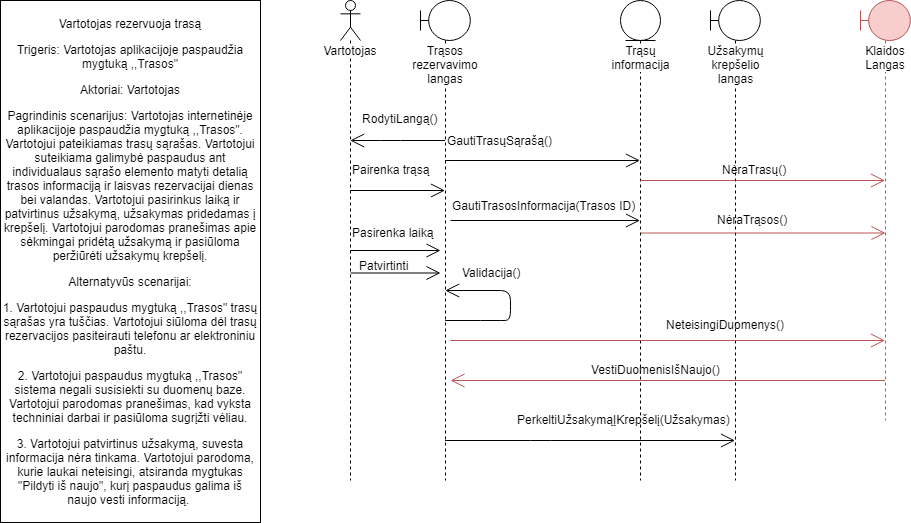
\includegraphics[width=0.75\textwidth]{seq8.png}
    				\caption{Vartotojas rezervuoja trasą}
    				\label{fig:VartotojoUseCasel}
			\end{figure}

			\begin{figure}[h]
    				\centering
    				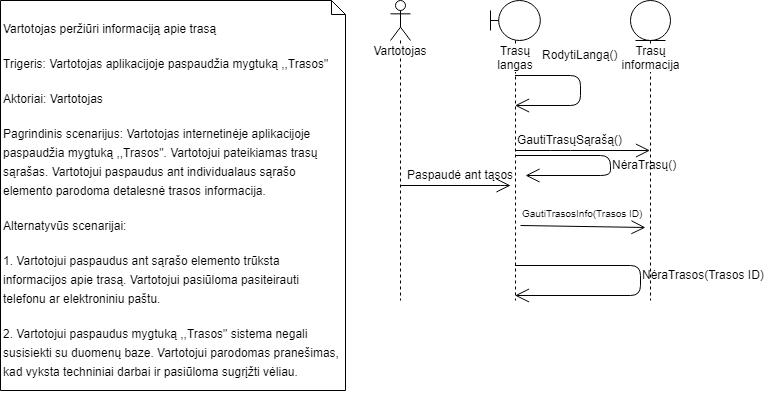
\includegraphics[width=0.75\textwidth]{seq9.png}
    				\caption{Vartotojas peržiūri trasos informacijos}
    				\label{fig:Vartotojas peržiūri trasos informacijos}
			\end{figure}

			\begin{figure}[h]
    				\centering
    				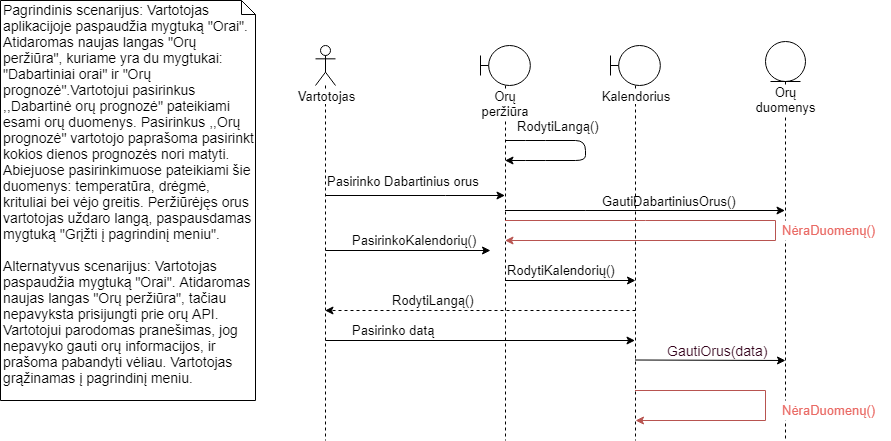
\includegraphics[width=0.75\textwidth]{seq10.png}
    				\caption{Vartotojas peržiūri orų prognozę}
    				\label{fig:Vartotojas peržiūri orų prognozę}
			\end{figure}

			\begin{figure}[h]
    				\centering
    				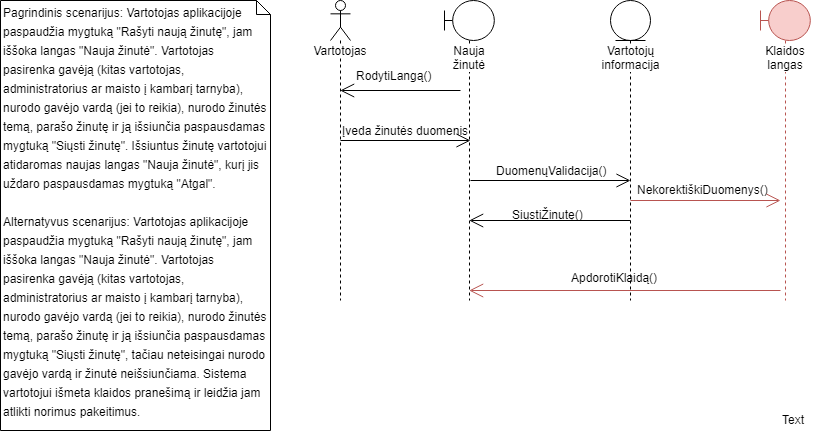
\includegraphics[width=0.75\textwidth]{seq11.png}
    				\caption{Vartotojas rašo žinutę}
    				\label{fig:Vartotojas rašo žinutę}
			\end{figure}

			\begin{figure}[h]
    				\centering
    				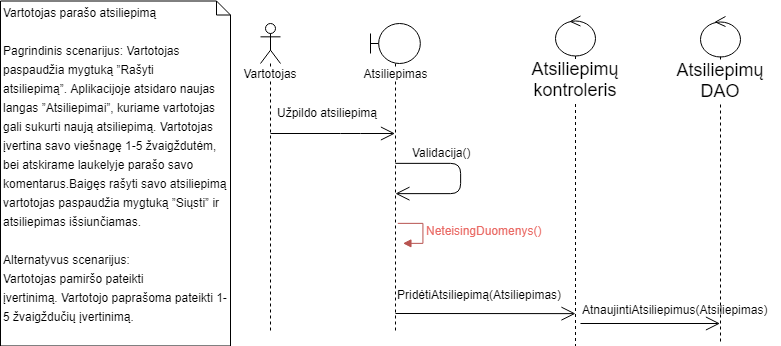
\includegraphics[width=0.75\textwidth]{seq12.png}
    				\caption{Vartotojas rašo atsiliepimą}
    				\label{fig:Vartotojas rašo atsiliepimą}
			\end{figure}

			\begin{figure}[h]
    				\centering
    				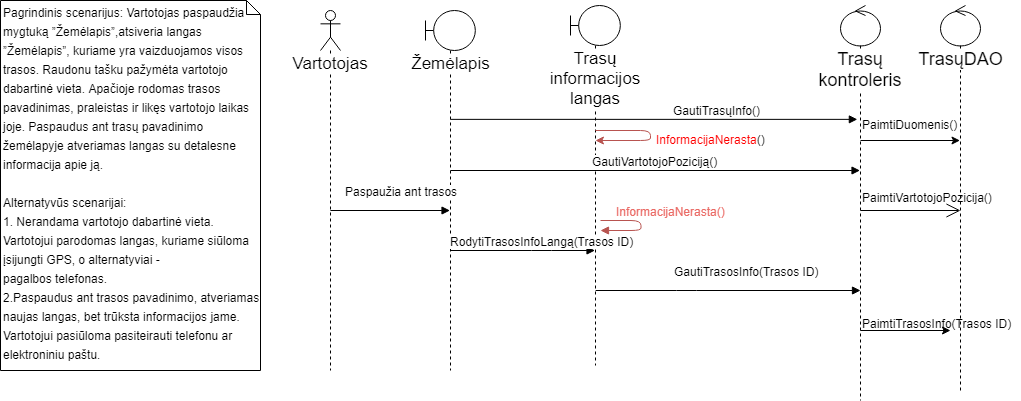
\includegraphics[width=0.75\textwidth]{seq13.png}
    				\caption{Vartotojas peržiūri žemėlapį}
    				\label{fig:Vartotojas peržiūri žemėlapį}
			\end{figure}

			\begin{figure}[h]
    				\centering
    				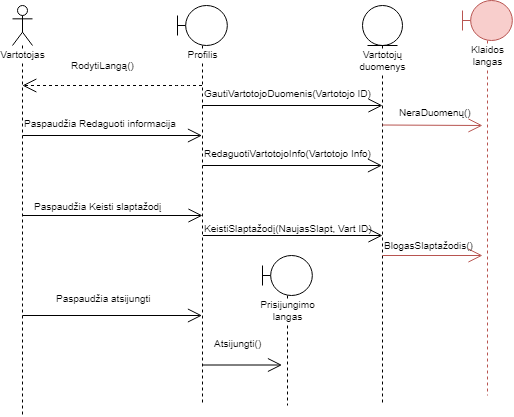
\includegraphics[width=0.75\textwidth]{seq14.png}
    				\caption{Vartotojas keičia asmeninius duomenis}
    				\label{fig:Vartotojas keičia asmeninius duomenis}
			\end{figure}

\section{Klasių diagrama}

\section{Detalaus projekto peržiūra}
	\subsection{Peržiūra}
	\subsection{Atsekamumas}

\section{Testavimo planas ir scenarijai}
	\subsection{Programinių vienetų testai}
	\subsection{Sistemos užduočių testai}

\section{Sistemos techninė architektūra}
	\subsection{Sistemos komponentų diagrama}
			\begin{figure}[h]
    				\centering
    				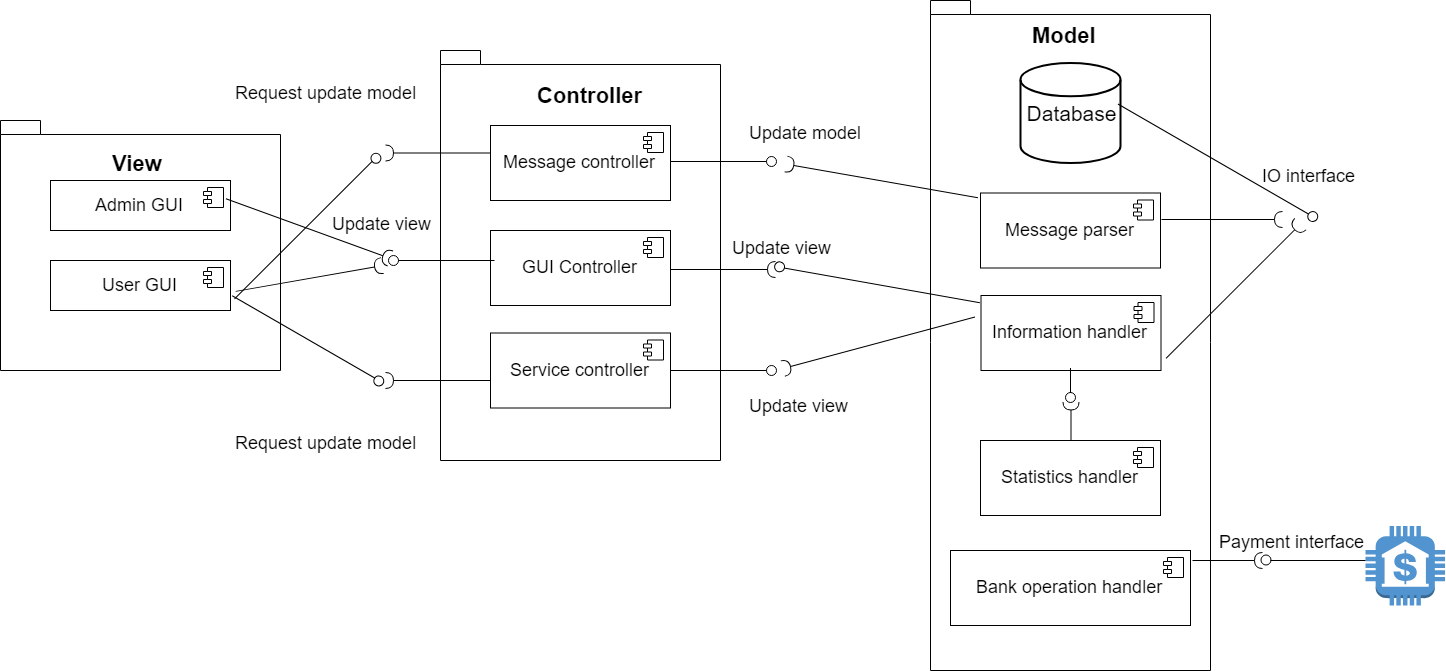
\includegraphics[width=0.75\textwidth]{KomponentuDiagrama.png}
    				\caption{Komponentų diagrama}
    				\label{fig:Komponentų diagrama}
			\end{figure}

	Sistema išskaidyta į 3 sluoksnius, View, Controller ir Model. View sluoksnyje talpiname vartotojoir administratoriaus grafinius interfeisus, kurie bendrauja su Controller esančiais komponentais. Controller sluoksnyje esantys komponentai yra tarpiniai tarp grafinio interfeiso ir back-end. Komponentai, esantys jame, gavę grafinio interfeiso signalus juos apdoroja ir kreipiasi į Model, kuriame esantys komponentai pagrinde skirti duomenų bazės redagavimui. Norint atvaizduoti atnaujintą informaciją vartotojui, Model esantys komponentai perduoda informaciją į Controller ir pastarasis perduoda informaciją View, kur ją išvysta vartotojas.
	\subsection{Išdėstymo diagrama}
			\begin{figure}[h]
    				\centering
    				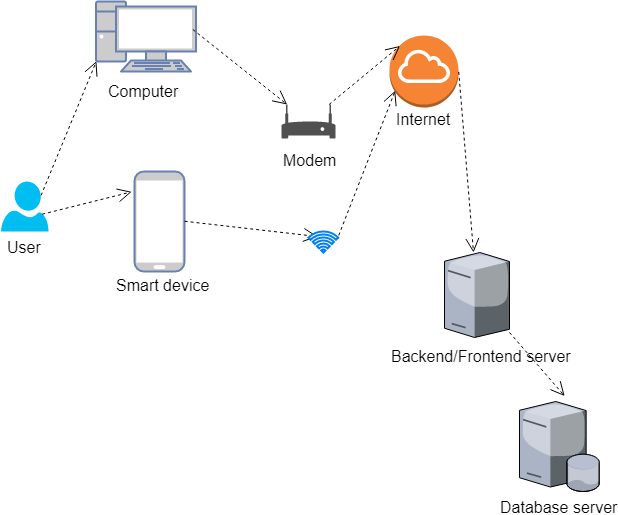
\includegraphics[width=0.75\textwidth]{Deployment.png}
    				\caption{Komponentų diagrama}
    				\label{fig:Komponentų diagrama}
			\end{figure}

\section{Sistemos realizacija}
	\subsection{Duomenų bazės schema}
	\subsection{Pradiniai programų kodai ir aprašas}

\section{Reikalavimų specifikacija}

\section{Žodynas}


\end{document}